% !TEX program = tectonic
% The Detector Was the Result — Farina 2026
% Build: tectonic detector_paper_farina_2026.tex
\documentclass[11pt,letterpaper]{article}

\usepackage[letterpaper,margin=1in]{geometry}
\usepackage{setspace}
\onehalfspacing

\usepackage[T1]{fontenc}
\usepackage{lmodern}
\usepackage[utf8]{inputenc}
\usepackage{microtype}
\usepackage{textcomp}

\usepackage{amsmath,amssymb}
\usepackage{siunitx}

\usepackage{booktabs}
\usepackage{array}
\usepackage{graphicx}
\usepackage{float}
\usepackage{caption}
\captionsetup{font=small,labelfont=bf,labelsep=period,skip=6pt}

\usepackage[round,authoryear]{natbib}
\bibliographystyle{plainnat}

\usepackage[dvipsnames]{xcolor}
\definecolor{linkcol}{rgb}{0.0,0.20,0.45}
\usepackage[colorlinks=true,linkcolor=black,citecolor=black,
            urlcolor=linkcol,breaklinks=true]{hyperref}
\usepackage{url}

\usepackage{fancyhdr}
\pagestyle{fancy}
\fancyhf{}
\fancyhead[L]{\small\itshape The Detector Was the Result}
\fancyhead[R]{\small Farina 2026}
\fancyfoot[C]{\thepage}
\renewcommand{\headrulewidth}{0.4pt}
\renewcommand{\footrulewidth}{0pt}

\usepackage{titlesec}
\titleformat{\section}{\large\bfseries}{\thesection.}{0.6em}{}
\titleformat{\subsection}{\normalsize\bfseries}{\thesubsection}{0.6em}{}

\usepackage{enumitem}
\setlist{itemsep=2pt,topsep=4pt}
\setlength{\parskip}{4pt}
\setlength{\parindent}{1.5em}

\usepackage{listings}
\lstset{basicstyle=\ttfamily\small,frame=single,framesep=4pt,
        backgroundcolor=\color{black!3},breaklines=true,
        xleftmargin=0pt,aboveskip=8pt,belowskip=8pt}

\title{\textbf{The Detector Was the Result:\\
Eight Measurement Artifacts, and a Question\\
That Cannot Be Asked This Way}}
\author{%
  Micka\"el Farina\\
  \small Independent Researcher, Marbella, Spain\\
  \small \href{mailto:mikarina@avadigital.ai}{\texttt{mikarina@avadigital.ai}}
}
\date{\small Preprint \textperiodcentered\ August 2026}

\begin{document}
\maketitle
\thispagestyle{fancy}

\begin{abstract}
\noindent
\textbf{\upshape Abstract.} We report a simulation result, its
retraction, and the audit that produced both. A protocell model of
1{,}845 Monte Carlo runs appeared to show that division regularity
(``Clock'') precedes spatial organization (``Map'') without exception:
100\,\% consistency, binomial $p \approx 10^{-146}$. The result was
reproducible, survived a twelve-condition parameter ablation,
replicated across two geometries, and passed three rounds of external
adversarial review. It was an artifact. The phase detector latched the
second predicate only after the first had latched, so no other outcome
was reachable; the reported inter-phase delay equalled the sampling
interval exactly; and the first predicate's latch time tracked the
moment its statistic became \emph{computable} rather than any change in
the system. We document eight such defects, each sufficient alone to
produce the headline. We then validate the corrected measurement by
planting a known ordering in the model's physics and recovering it
($\rho = +0.96$; Clock-first rising from 2.6\,\% to 100\,\% across the
planted sweep), so that the corrected figure --- the ordering holds in
$\approx$1\,\% of runs --- is a measurement rather than a blind spot.
Three attempts to rescue the hypothesis follow. The third is the
result: a Clock metric constructed specifically to have no definedness
floor becomes defined \emph{later} than the metric it replaces. A
buffer sweep shows why. The replacement only measures regularity at all
once its history spans $\sim$9 division periods ($\rho = -0.46$,
$p = 0.003$ out of sample; shorter buffers return the wrong sign), and
its definedness time equals that buffer length identically --- so the
earliest a valid Clock reading can exist is $\sim$24{,}000 ticks,
against a spatial metric defined by $\sim$150. Measuring the regularity
of a slow periodic process requires observing several of its periods;
measuring correlation in a fast field does not. The asymmetry that
produced the original artifact is therefore substantially a
time--frequency constraint rather than an implementation error, and the
ordering question is malformed as posed: comparing first-crossing times
measures the ratio of two intrinsic timescales, not the dynamics.
Ordering claims of this kind must be tested by intervention instead. We
release an automated checklist that recovers all eight defects from
source, and record that its authors committed the same class of error
six times while writing this paper --- the last of them an instrument
validated by eye from an insignificant correlation, in the section
arguing that unvalidated instruments are worthless.

\vspace{6pt}
\noindent\textbf{Keywords:} artificial life; protocell models;
measurement artifact; phase detection; Simpson's paradox;
reproducibility; self-correction
\end{abstract}

% ════════════════════════════════════════════════════════════════════
\section{Introduction}

\subsection{A result that looked strong}

In April 2026 we published a protocell simulation --- in the tradition
of minimal-cell and vesicle-replication modelling
\citep{szostak2001,hanczyc2003} and of the open problems programme in
artificial life \citep{bedau2000} --- reporting that the emergence of
biological agency follows a mandatory order: temporal
regularity of division (the \emph{Clock}) precedes persistent spatial
organization (the \emph{Map}), which precedes thermodynamic selection
(the \emph{Engine}). Across 1{,}845 Monte Carlo runs in which both
transitions occurred, the Clock preceded the Map in every single one.

By the conventional signals, the result was strong. Perfect
separation. A binomial $p$-value of $8.01 \times 10^{-146}$. Replication
across a one-dimensional ring and a two-dimensional spherical manifold.
Robustness across a twelve-condition parameter ablation spanning
factor-of-two perturbations in lipid supply, reaction--diffusion noise,
growth perturbation, and stability window. Full public code and data
from the day of posting. Three subsequent rounds of adversarial review
by frontier language models, each of which found real problems and
prompted genuine improvements, and none of which found what follows.

The result was an artifact. This paper is the account of how it was
produced, how it was found, and what the finding turned out to be worth.

\subsection{Thesis: reproducibility is not validity}

Every number in the original paper reproduces. We re-ran the archived
seeds during this audit and obtained identical phase-transition ticks a
year later. The code does what it says. The data are real. Nothing was
fabricated and nothing was tuned.

That is precisely the problem. A quantity can reproduce to fifteen
significant figures and still be a number \emph{of the wrong thing}.
The reported inter-phase delay of 243 ticks is a correct arithmetic
summary of a distribution whose median is 50 --- and 50 was the
sampling interval. The reported Clock latch time is a correct readout of
when a statistic first returned a value --- and that value was
unavailable until a cell had divided four times.

We take this as the paper's thesis. Reproducibility protects against
fabrication and against transcription error. It offers no protection at
all against an instrument that cannot emit the answer you are looking
for. The distinction is not new --- computational reproducibility has
long been argued to be necessary rather than sufficient
\citep{peng2011,stodden2016}, and \citet{leek2015} make the sharper
point that reproducible research can still be wrong --- but the case
below is an unusually complete worked example, in which every number
reproduces and the headline is nonetheless an artifact.

\subsection{Contributions}

\begin{enumerate}
\item Eight documented measurement defects in a published result, each
      independently sufficient to produce the headline, with the
      corrected figures.
\item A validated corrected measurement: we plant a known ordering in
      the physics and demonstrate the corrected method recovers it,
      so that our nulls are informative rather than blind.
\item The demonstration that the underlying question is malformed as
      posed --- a time--frequency constraint, not a defect --- and the
      constructive replacement.
\item \texttt{detector\_audit.py}, an eight-check runner that recovers
      all eight defects from source and archived data with no audit
      knowledge encoded.
\item A record of six errors of the same class committed by the
      authors \emph{during} the audit, which we take to be the most
      instructive part of the account.
\end{enumerate}

\subsection{Status of the original paper}

The original preprint (SSRN 6593781, April 2026) remains posted with a
correction notice attached rather than being removed. We took that
decision deliberately. The paper's data and code are the evidence for
this one, the defects are only legible against the original text, and
silent withdrawal would leave the eleven months in which the claim
circulated unaccounted for. The correction notice withdraws the central
result explicitly and in full, lists all eight defects with corrected
figures, and links to the audit materials. Readers arriving at the
original by citation reach the correction before the abstract.

Two companion papers cannot be treated the same way. Neither the
Vesicle Division nor the Engine study has surviving source code on any
machine we control, so their headline figures --- a division-interval
$\mathrm{CV} = 0.06$ and an effect size $g = 4.07$ --- cannot be checked
for the circularity documented here. We do not assert those results are
wrong. We report that we are unable to verify them, which given what
follows we consider the more useful statement.

% ════════════════════════════════════════════════════════════════════
\section{The model and the original claim}

\subsection{Dynamics}

The model follows a population of protocells. Each carries a
Gray--Scott reaction--diffusion field \citep{gray1983,pearson1993} on
its membrane (a 24-node ring in 1D; a 642-vertex icosphere with a
cotangent Laplace--Beltrami operator in 2D), grows by lipid accretion at
a rate set by a shared resource pool, and divides by geometric
instability once its reduced volume crosses a noisy threshold --- the
``Adder'' mechanism \citep{taheri2015,campos2014}. Pattern
stability $S$ couples multiplicatively into metabolic efficiency,
nutrient uptake, and maintenance cost.

Division timing depends on membrane geometry and resource availability.
It does not depend on the reaction--diffusion field. This one-way
coupling was deliberate: it was intended to make the ordering claim
non-circular.

\subsection{The phase predicates}

Three thresholded predicates define the phases:

\begin{itemize}
\item \textbf{Clock (B)}: population-mean division-interval coefficient
      of variation $\mathrm{CV} < 0.25$
\item \textbf{Map (C)}: population-mean pattern stability
      $\bar{S} > 0.25$
\item \textbf{Engine (D)}: $\bar{S} > 0.35$, $\mathrm{CV} < 0.3$, and
      generational depth $\geq 5$
\end{itemize}

Each predicate, once satisfied, latches. The tick of first latching is
recorded, and the ordering claim compares those ticks.

\subsection{The published result}

\begin{table}[H]
\centering
\caption{The original headline, as published.}
\begin{tabular}{lr}
\toprule
Quantity & Reported value \\
\midrule
Clock before Map & 1{,}845 / 1{,}845 (100\,\%) \\
Binomial $p$ (1D) & $8.01 \times 10^{-146}$ \\
Binomial $p$ (2D) & $2.49 \times 10^{-60}$ \\
Mean Clock$\to$Map delay (1D) & $243 \pm 2{,}319$ ticks \\
Mean Clock$\to$Map delay (2D) & $56 \pm 41$ ticks \\
Hedges' $g$ (1D) & 9.41 \\
Hedges' $g$ (2D) & 3.27 \\
\bottomrule
\end{tabular}
\end{table}

% ════════════════════════════════════════════════════════════════════
\section{The audit}

\subsection{Method}

The audit did not re-read the manuscript. It re-ran the simulation under
added instrumentation, on the archived seeds, and compared what the
instruments reported against what the dynamics did. Every defect below
was found by running code against code, not by reasoning about the
argument.

\subsection{Defect 1 --- the detector could not fail}

The phase detector contains the following condition:

\begin{lstlisting}
if ph.B and ph.B_tick < tick and not ph.C and mean_s > PHASE_C_S:
    ph.C = True
\end{lstlisting}

The Map predicate latches only if the Clock predicate latched at a
\emph{strictly earlier} tick. A run in which the Map preceded the Clock
is not merely unlikely under this detector; it is unreachable. The
reported 100\,\% was the only value the function could return.

Two consequences follow. First, the proportion carries no evidence about
the dynamics. Second, both reported significance tests are computed
against nulls that no possible run could have violated: the binomial
tests $p = 0.5$ random ordering, and the Wilcoxon tests whether the delay
exceeds zero, when the gate guarantees a delay of at least one sampling
interval. A $p$-value against an unreachable null is not weak evidence.
It is not evidence.

We re-instrumented both engines to log \emph{ungated} first crossings:
each predicate evaluated at every measurement tick, independently, with
neither able to suppress the other. Default behaviour was unchanged
(verified by exact reproduction of archived phase ticks on seeds 0, 1,
and 2).

\subsection{Defect 2 --- the delay is the sampling interval}

The reported mean delay was 243 ticks. The median is 50. The
interquartile range is $[50, 50]$ --- zero width. In 1D, 434 of 482 runs
(90.0\,\%) recorded a delay of exactly 50 ticks; in 2D, 193 of 198
(97.5\,\%). Fifty ticks was the sampling interval.

Re-running 100 seeds at 1-tick sampling, the gated delay collapses to
exactly 1 tick in 91 of the 97 runs in which both predicates latched
(93.8\,\%; in the remaining three seeds the Map predicate never
latched). The delay is not a property of the system. It is the
measurement grid.

\subsection{Defect 3 --- the latch time is a definedness floor}

The Clock statistic is undefined until a cell has accumulated three
division intervals, which requires four completed divisions; until then
it returns a sentinel value of 1.0, above every candidate threshold.
The Clock predicate therefore \emph{cannot} fire before that point,
whatever the dynamics do.

\begin{table}[H]
\centering
\caption{The reported Clock latch coincides with the tick at which the
Clock statistic first becomes computable. Medians over the full
archive ($n = 500$ in 1D, $n = 200$ in 2D).}
\begin{tabular}{lrr}
\toprule
& First tick CV computable & Reported Clock latch \\
\midrule
1D & 4{,}200 & 4{,}200 \\
2D & 4{,}900 & 4{,}900 \\
\bottomrule
\end{tabular}
\end{table}

An earlier draft reported 4{,}250/4{,}250 and 4{,}950/4{,}975 here.
Those were medians over a 120-run subset; the figures above are the full
archive. The agreement is exact in both geometries at full $n$. All such
medians lie on a 50-tick grid, because 50 ticks is the sampling
interval; a median quoted off that grid is an average of two adjacent
grid points across an even number of runs, not an observation. An
earlier draft reported 4{,}825 for the 1D figure on that basis.

Meanwhile the Map statistic exceeds its threshold at median tick 1{,}400
(1D) and 1{,}300 (2D) --- before the Clock statistic exists at all. The
Map predicate crossed before CV was computable in 115 of 116 archived 1D
runs and 118 of 118 2D runs.

We initially catalogued this as a straightforward implementation error.
Section~\ref{sec:redesign} shows that assessment was only half correct.

\subsection{Defect 4 --- the mean is three runs}

Total delay mass across the 482 1D runs is 117{,}100 ticks. Three
runs --- seeds 171, 294 and 361, with delays of 38{,}400, 32{,}000 and
10{,}450 ticks --- account for 80{,}850 of it, or 69.0\,\%. Excluding
them, the mean falls from 242.9 to 75.7, within 26 ticks of the floor.
The reported standard deviation, 2{,}319, is roughly ten times its own
mean.

The archived \texttt{paper\_data.json} already contained
\texttt{delay\_C\_minus\_B/median = 50.0} in the same object as the mean.
The correction was available in the paper's own data file from the day
of posting.

\subsection{Defect 5 --- the denominator double-counts}

The headline denominator of 1{,}845 pools three studies: 482 runs from
the 1D main study, 1{,}165 from the ablation grid, and 198 from 2D.

The ablation is one-at-a-time: four parameters at three levels each,
where one level of each sweep \emph{is} the baseline. Reporting the
shared baseline in all four rows is standard practice and is not the
error. The error was summing all twelve rows to obtain a total. All four
baseline rows are identical to the last decimal place --- mean B tick
4416.0, mean C tick 4518.556701030928, mean final $S$
0.7521093934657955 --- because they are the same 97 runs. Counted once
per parameter sweep, those 97 runs enter the total four times instead of
once, contributing $97 \times 3 = 291$ redundant counts.

Distinct runs: $1{,}165 - 291 = 874$ from the ablation, so
$482 + 874 + 198 = \textbf{1{,}554}$, not 1{,}845.

\subsection{Defect 6 --- the effect sizes, and the story told about them}
\label{sec:effectsize}

This is the centrepiece, because it is the only defect where we did not
merely make an error --- we explained one.

Hedges' $g$ is computed on \texttt{final\_pop}, grouped by
\texttt{final\_mean\_s}. But $S$ multiplies uptake, efficiency, and
maintenance directly (bonus coefficients 0.12, 0.70 and 0.35), so it
causally determines final population. Grouping on $S$ and measuring
population largely measures our own chosen coupling constants.

Worse, the group sizes are degenerate. Recomputing from the archived
summaries with the published thresholds:

\begin{table}[H]
\centering
\caption{Effect-size group sizes, recomputed. Both published values
reproduce exactly.}
\begin{tabular}{lrrrr}
\toprule
Geometry & Organized ($\bar S > 0.3$) & Disorganized ($\bar S < 0.1$)
& $g$ & Published \\
\midrule
1D & 482 & 18 & 9.4124 & 9.41 \\
2D & 198 & \textbf{2} & 3.2737 & 3.27 \\
\bottomrule
\end{tabular}
\end{table}

The 2D effect size rests on a comparison arm of \emph{two runs}. No 2D
run falls between the thresholds, so the split is degenerate rather than
merely unbalanced.

The repository additionally reports a ``combined'' $g = 6.34$. That
value is exactly $(9.41 + 3.27)/2$: the arithmetic mean of two effect
sizes, which is not a valid pooling under any convention, and one of
whose inputs has $n = 2$.

And in \S4.3 of the original paper we explained the lower 2D value as
reflecting ``more spatial degrees of freedom.'' An artifact appeared, and
we reached for physics to account for it rather than checking
\texttt{len()}. We consider this the single most instructive sentence in
the original manuscript.

\subsection{Defect 7 --- gate dependence is systematic}

Auditing all nineteen reported quantities by tracing each computation
path in source, nine depend directly on detector outputs and a tenth
depends on one indirectly. Phase-D success rates
(90\,\% versus 79\,\% across lipid supply) are withdrawn as rates,
because they count a latched state whose latch time is set by the
definedness floor. Only the \emph{direction} of the difference survives,
and it survives for a specific reason: two independent confounds --- more
post-transition time available at high lipid supply ($+5{,}049$ ticks),
and greater generational depth (4.87 versus 4.74) --- both predict the
opposite sign to the one observed.

The audit also demoted two results we had ourselves placed in the
surviving column, both from the section added in response to external
review. All four results in that section are withdrawn or demoted; the
section does not survive as physics. Two survive as arithmetic with
their causal readings withdrawn, because their measurement windows were
anchored on \texttt{phase\_C\_tick} --- which Defect 3 established is not
when the Map latched.

\subsection{Defect 8 --- a sign reversal}

The reported correlation between division period and pattern stability
was $\rho = +0.43$ pooled across lipid conditions. Stratified:

\begin{table}[H]
\centering
\caption{A Simpson's paradox. Pooling reverses the sign.}
\label{tab:simpson}
\begin{tabular}{lrr}
\toprule
Stratum & $n$ & $\rho(T_{\mathrm{div}}, S)$ \\
\midrule
Lipid supply 0.008 & 100 & $-0.5970$ \\
Lipid supply 0.015 & 100 & $-0.7396$ \\
Lipid supply 0.025 & 100 & $-0.7537$ \\
\midrule
Pooled (as published) & 300 & $\mathbf{+0.4278}$ \\
\bottomrule
\end{tabular}
\end{table}

Lipid supply moves both variables at once, so they covary positively
across conditions; within a fixed supply, slower-dividing runs reach
\emph{lower} stability. The published value has the wrong sign. The
structure is the classical one \citep{simpson1951,blyth1972}.

\subsection{The corrected figure}

Measured without the gate, the Clock precedes the Map in approximately
1\,\% of runs: $1/97 = 1.0$\,\% by 1-tick resampling (100 seeds, of
which 97 latched both predicates), 0.7\,\% by a threshold grid over
archived timeseries ($n = 150$), and 0.0\,\% in 2D across all nine cells
of a $3 \times 3$ threshold grid. Two independent methods, in close
agreement.

We note that the 97 here and the 97 baseline runs of Defect 5 are an
arithmetic coincidence of two unrelated experiments, not the same
quantity.

% ════════════════════════════════════════════════════════════════════
\section{Validating the corrected instrument}
\label{sec:validate}

\subsection{Why a null from an unvalidated instrument is worthless}

At this point the audit had produced a series of null and negative
results. None of them meant anything yet.

An instrument that cannot detect an ordering will report no ordering
whether or not one exists. Reporting nulls from an uncalibrated
detector is the same class of error as the original paper, pointed in
the opposite direction --- and we had committed it for several weeks
without noticing.

\subsection{Planting a known ordering}

We planted an ordering in the \emph{physics}, not the detector: pattern
stability is held at zero for every cell until tick $T$, making spatial
organization physically impossible before then. No involvement of the
detector, the gate, or the Clock statistic; ground truth known exactly.
A wall-clock plant was chosen deliberately, since gating the plant on
division regularity would inherit the very floor under test.

\begin{figure}[H]
\centering
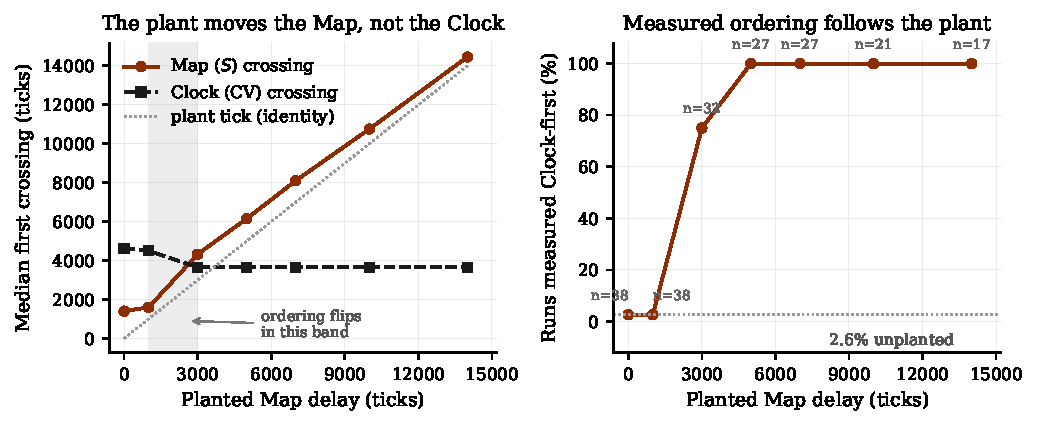
\includegraphics[width=\textwidth]{figures/fig1_positive_control.pdf}
\caption{The positive control. \textbf{Left:} median first-crossing
tick of each predicate against planted Map delay. The Map crossing
tracks the plant (dotted identity line); the Clock crossing does not
follow it, but does shift from 4{,}625 to 3{,}650 once the plant bites
--- the non-orthogonality noted below, and the reason ordering is judged
within-run rather than against a fixed Clock time. \textbf{Right:}
fraction of runs measured Clock-first, rising from 2.6\,\% to 100\,\%
as the plant crosses the natural Clock time. Annotated $n$ is the number
of runs in which both predicates latched, which falls at large plants.}
\label{fig:control}
\end{figure}

\begin{table}[H]
\centering
\caption{Positive control. 280 runs, seven plant levels $\times$ 40
seeds. The measured ordering flips as the plant crosses the natural
Clock time for this configuration ($\sim$4{,}250 ticks; the archive
median of 4{,}200 in Defect 3 is the same quantity at a different run
length and seed count).}
\begin{tabular}{rrrr}
\toprule
Plant tick & Median measured Map crossing & Clock-first & Map after plant \\
\midrule
0 (none) & 1{,}400 & 2.6\,\% & --- \\
1{,}000 & 1{,}600 & \textbf{2.6\,\%} & 100\,\% \\
3{,}000 & 4{,}325 & 75.0\,\% & 100\,\% \\
5{,}000 & 6{,}150 & 100\,\% & 100\,\% \\
7{,}000 & 8{,}100 & 100\,\% & 100\,\% \\
10{,}000 & 10{,}750 & \textbf{100\,\%} & 100\,\% \\
14{,}000 & 14{,}450 & 100\,\% & \textbf{100\,\%} \\
\bottomrule
\end{tabular}
\end{table}

All three pre-registered criteria pass: recovery
($\rho = +0.9560$, required $> +0.8$; $p < 10^{-100}$, computed over
200 runs at the cell level and quoted here only as a bound, since at
this effect size the exact value is an artifact of the sample size
rather than evidence about the ordering);
flip (2.6\,\% $\to$ 100\,\%, required $< 20$\,\% and $> 80$\,\%);
and fidelity (100\,\%, required $> 90$\,\%).

\subsection{Consequence}

The corrected measurement detects a real ordering when one exists, and
the crossover falls where it should. The $\approx$1\,\% figure is
therefore a measurement of the model's dynamics, not a blind spot. It
also disposes of the obvious objection --- that the method is biased
toward Map-first --- since planting the ordering flips it to 100\,\%
Clock-first without hesitation.

Three caveats belong in the record. Runs in which both predicates fired
fall from 38/40 at no plant to 17/40 at the largest plant, because
larger plants leave less run time for stability to recover; the
recovery correlation therefore rests on 200 of 280 runs. The plant
is not perfectly orthogonal: suppressing $S$ also suppresses the
$S$-linked metabolic bonuses, shifting division dynamics. Ordering is
consequently judged within each run on that run's own two crossings,
never against an assumed Clock time.

The third caveat bounds what the control licenses. It plants
\emph{Clock-before-Map} by delaying the Map, and demonstrates recovery
in that direction only. We did not run the mirror experiment --- an
accelerated Clock, or a delayed Clock against an undisturbed Map ---
because the Clock statistic's definedness floor is precisely the
quantity under investigation, so any plant acting on it would be
confounded with the effect being measured. The control therefore
establishes that the method is not blind to Clock-first orderings when
they exist. It does not establish symmetric sensitivity, and the
$\approx$1\,\% figure should be read as an upper bound on our ability to
detect Clock-first rather than as a two-sided measurement.

% ════════════════════════════════════════════════════════════════════
\section{Three attempts to rescue the hypothesis}
\label{sec:rescue}

The underlying physical claim --- that temporal regularity enables
spatial organization --- had still never been tested, only mismeasured.
We made three attempts.

\subsection{Intervention}

We imposed division timing externally, drawing intervals from
$\Gamma(1/c^2,\, T c^2)$, which has mean $T$ and coefficient of variation
$c$ exactly ($c = 0$ deterministic, $c = 1$ Poissonian). Division
regularity becomes a control variable rather than an estimate, and
steady-state $S$ is measured over the final 20\,\% of each run with no
detector and no CV estimator anywhere in the causal path. Grid: nine
CV levels $\times$ six periods $\times$ 25 seeds = 1{,}350 runs.

Only two of the six periods are physically valid: below the model's
natural period under this forced-division configuration
($\sim$3{,}170 ticks) forced division splits cells before they have
grown, reaching 79.4\,\% premature splits at $T = 1600$ and 100\,\% at
$T = 200$. (Elsewhere in this paper the natural period is given as
$\sim$2{,}500 ticks. The two figures describe different experiments ---
the 1D main study at 80{,}000 ticks under natural division, and this
forced-division grid --- and are not in conflict. Every period quoted in
this paper is configuration-specific and we label it as such from here
on.) Within the valid window:

\begin{table}[H]
\centering
\caption{Steady-state $S$ against imposed division regularity, physical
periods only ($n = 450$).}
\begin{tabular}{lrrrrrrrrr}
\toprule
Imposed CV & 0.0 & 0.05 & 0.10 & 0.15 & 0.20 & 0.30 & 0.50 & 0.80 & 1.0 \\
\midrule
Mean $S$ & 0.760 & 0.664 & 0.687 & 0.710 & 0.700 & 0.702 & 0.726 & 0.773 & 0.781 \\
\bottomrule
\end{tabular}
\end{table}

$\rho(\mathrm{CV}, S) = +0.2196$ ($p = 2.6 \times 10^{-6}$): stability
\emph{rises} with irregularity, opposite to prediction. A one-sided
Mann--Whitney test of the hypothesis' own direction (regular
$>$ irregular) returns $p = 1.0$.

That monotone summary misdescribes the table it summarises. The
response is not monotone but U-shaped: $S$ falls from 0.760 at
$\mathrm{CV} = 0$ to a minimum of 0.664 at $\mathrm{CV} = 0.05$, then
rises to 0.781 at $\mathrm{CV} = 1.0$. The perfectly regular condition
is the second-\emph{highest} in the row, not the lowest, so a rank
correlation computed across the whole range averages a decrease and an
increase and reports the net. We flag this rather than resolve it: the
$\mathrm{CV} = 0$ point is also the condition with 27.3\,\% extinction
(\S\ref{sec:survives}), so the surviving runs there are a survivorship-
filtered subpopulation and the point is not comparable to its
neighbours on equal terms. The honest statement is that imposed
regularity does not raise stability anywhere in this grid, and that the
single number $+0.2196$ should not be read as a dose--response.

The effect survives three of four pre-registered confound checks,
including a matched-interval control that excludes the obvious
alternative explanation (the Gamma right tail): the association persists
within interval-matched quintiles with only 19\,\% attenuation
($\rho = +0.169$ unconditional versus $+0.137$ within bins,
$n = 139{,}715$). It fails the fourth: the fraction of barely-dividing
cells rises from 44.0\,\% to 56.2\,\% across the sweep, against a
pre-registered threshold of 10 percentage points. The hypothesis is
therefore neither confirmed nor refuted by this experiment.

We note that we did not move the threshold. The primary confound was
cleared cleanly and the miss was 2.3 points on a criterion we had set
ourselves.

\subsection{Reformulation}

Perhaps the theory named the wrong variable. Variance per se has no
obvious mechanism; short intervals do. If patterns need
$\sim$1{,}350 ticks to consolidate, what should matter is the
\emph{minimum} uninterrupted interval, with regularity mattering only
insofar as it produces short ones. This also predicts the flat result
above, since raising Gamma CV adds both short and long intervals.

Pre-registered and run on natural division ($n = 153{,}133$
cell-observations): $\rho(\text{min interval}, S) = +0.3844$ pooled,
which passes the criterion. Stratified by division count, it does not:

\begin{table}[H]
\centering
\caption{The third Simpson's paradox. The pooled association vanishes
or inverts within strata.}
\begin{tabular}{lrr}
\toprule
Division intervals & $n$ & $\rho(\text{min interval}, S)$ \\
\midrule
1--2 & 28{,}266 & $+0.0918$ \\
3--4 & 25{,}745 & $-0.1525$ \\
5--8 & 50{,}375 & $-0.0495$ \\
9+ & 48{,}747 & $-0.0840$ \\
\midrule
Pooled & 153{,}133 & $\mathbf{+0.3844}$ \\
\bottomrule
\end{tabular}
\end{table}

Cells that barely divided have both an upward-biased minimum and an
undisturbed high stability, so pooling manufactures the correlation. The
pre-registered disqualifier fires, and the secondary arm (forced
division) gives $\rho = -0.1484$ pooled, \emph{strengthening} to
$-0.3463$ under stratification --- the mirror image, and therefore not an
artifact. Both arms agree that longer minimum intervals do not produce
more stable patterns.

\subsection{Redesign, and what it revealed}
\label{sec:redesign}

The remaining possibility was that the instruments themselves were
mismatched. We therefore attempted to replace the Clock metric with one
having no definedness floor: the normalised autocorrelation of a cell's
own radius trajectory. A regularly dividing cell traces a sawtooth that
autocorrelates strongly at its period; an irregular one weakly. It
requires no divisions and is defined as soon as its buffer fills.

Any such metric must first pass a validity check: $\mathrm{clock}_r$
must correlate \emph{negatively} with CV across runs, since a more
regular divider should show both higher autocorrelation and lower
interval variance. A metric failing this is not measuring regularity,
whatever its definedness properties.

The first parameterisation failed it: with a 400-tick buffer searching
lags of 30--200 ticks, $\rho(\mathrm{clock}_r, \mathrm{CV}) = -0.190$,
$p = 0.241$ over 40 seeds. The division period in this configuration is
$\sim$2{,}550 ticks and the lag window could not reach it.

Widening the buffer to 6{,}000 ticks --- 2.4 division periods --- does
not fix it. Over 40 seeds that parameterisation gives
$\rho = +0.2162$, $p = 0.186$: still the wrong sign, still
insignificant. An earlier draft of this paper reported
$\rho = -0.2364$ for this arm and treated it as validation. That figure
is the first ten seeds, it was never significant ($p = 0.511$), and it
decays to $-0.0822$ ($p = 0.614$) at $n = 40$. Quoting a correlation
without its $p$-value to establish that an instrument works is the
error this paper is about, committed by us, in the section documenting
it. It is the sixth entry in \S\ref{sec:auditors}.

We therefore swept the buffer to ask whether \emph{any} span yields a
valid metric, holding the sample count fixed at 120 so that only the
span varies and reporting all four arms rather than stopping at the
first that passed.

\begin{figure}[H]
\centering
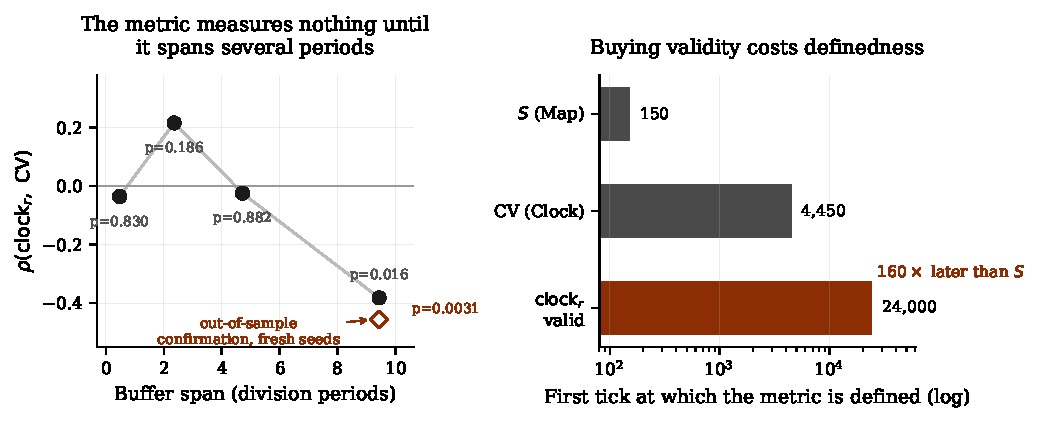
\includegraphics[width=\textwidth]{figures/fig2_definedness.pdf}
\caption{Why the redesign could not work. \textbf{Left:} validity of
$\mathrm{clock}_r$ against buffer span. The metric does not track
division regularity until its history spans $\sim$9 periods; the
2.4-period arm has the wrong sign. Filled points are the selection
sweep (black: does not clear the four-arm Bonferroni threshold); the
open diamond is the widest arm re-run on 40 fresh seeds.
\textbf{Right:} first tick at which each metric is defined, log scale.
Because definedness equals buffer length identically, the span that
buys validity is also the delay it costs.}
\label{fig:definedness}
\end{figure}

\begin{table}[H]
\centering
\caption{Buffer sweep, 40 seeds per arm, 40{,}000-tick runs. Validity
requires $\rho(\mathrm{clock}_r, \mathrm{CV}) < 0$ and significant.
Definedness equals buffer length in every arm.}
\begin{tabular}{rrrrrc}
\toprule
Buffer & Periods & Defined at & $\rho$ & $p$ & Valid \\
\midrule
1{,}200  & 0.47 & 1{,}200  & $-0.0354$ & 0.831 & no \\
6{,}000  & 2.36 & 6{,}000  & $+0.2162$ & 0.186 & no \\
12{,}000 & 4.71 & 12{,}000 & $-0.0245$ & 0.882 & no \\
24{,}000 & 9.43 & 24{,}000 & $\mathbf{-0.3822}$ & 0.016 & yes \\
\bottomrule
\end{tabular}
\end{table}

Two features carry the argument. \textbf{Definedness equals buffer
length exactly}, which is an identity rather than a result:
$\mathrm{clock}_r$ exists the moment its buffer fills. Whatever span
validity demands is therefore also the earliest the metric can exist.
And \textbf{the approach is not monotone} --- the 2.36-period arm has
the wrong sign and the 4.71-period arm is flat --- so we claim no smooth
relationship between span and validity, only that the intermediate arms
are uninformative at $n = 40$.

The widest arm's $p = 0.016$ does not clear a Bonferroni threshold of
$0.05/4 = 0.0125$. Since this is the paper's central claim, we re-ran
that arm on 40 seeds it had never been evaluated on:
$\rho = -0.4565$, $p = 0.0031$, with $\mathrm{clock}_r$ defined at tick
24{,}000 in 40 of 40 runs. That is a single pre-specified test of a
directional prediction and needs no correction.

\begin{table}[H]
\centering
\caption{Definedness of each metric, medians. The replacement metric,
in the only parameterisation shown to measure anything, is defined
$160\times$ later than the metric whose floor it was built to remove.}
\begin{tabular}{lrr}
\toprule
Metric & Defined at tick & Ratio to $S$ \\
\midrule
$S$ (Map) --- spatial correlation & 150 & --- \\
CV (original Clock) & 4{,}450 & $30\times$ \\
$\mathrm{clock}_r$, \emph{valid} parameterisation
  & \textbf{24{,}000} & $\mathbf{160\times}$ \\
\bottomrule
\end{tabular}
\end{table}

The pre-registered symmetry criterion required agreement within 20\,\%.
The observed ratio is $160\times$. The redesign did not merely fail to
remove the definedness floor it was built to remove; made valid, it
raised that floor by a further factor of five. Per the pre-registered
decision rule the downstream tests were not computed.

One property of the valid measurement must be stated rather than left
to be discovered. A 24{,}000-tick buffer is filled only by cells that
have lived 24{,}000 ticks, and daughters begin with an empty buffer
while mothers retain theirs, so $\mathrm{clock}_r$ is an average over an
age-selected subpopulation. This does not rescue the metric. A cell too
young to have a full buffer is exactly a cell whose period has not yet
been observed; the selection restates the constraint rather than
concealing it.

\subsection{The finding}

The redesign could not have worked, for a reason that has nothing to do
with implementation.

\textbf{To measure how regular a periodic process is, one must observe
several of its periods.} This is a time--frequency constraint of the
same family as the classical bound on simultaneous time and frequency
resolution \citep{gabor1946}, and it
is not specific to either estimator we tried. The CV of division
intervals needs four divisions. A radius autocorrelation, measured
here, needed $\sim$9 periods before it tracked regularity at all ---
two were not enough.

We state the scope of this claim carefully, because the obvious
objection is a good one. It applies to \emph{per-lineage} regularity
statistics: any quantity asking how evenly spaced one cell's events are
must wait for several of that cell's events. It does \emph{not} follow
that no Clock-like quantity can ever be defined early. A
\emph{cross-sectional} measure --- the dispersion of division phase
across a population at one instant --- is defined after roughly one
period rather than several, and we have not tested one. Our claim is
therefore bounded: the floor for per-lineage regularity is of order
several division periods, which for this model is $\sim$24{,}000 ticks
against $S$ at $\sim$150; whether a population-level phase statistic
narrows that gap is open, and we regard it as the most promising line
for anyone wishing to salvage a timing-based approach.

Meanwhile $S$ measures spatial correlation of a reaction--diffusion
field whose intrinsic correlation time is $\sim$40 ticks, and is
defined by $\sim$150. The asymmetry is therefore set by the ratio of
the two phenomena's intrinsic timescales --- a slow periodic process
against a fast field process --- and not by any choice we made.

\textbf{Defect 3 is consequently only half an error.} The specific
four-division floor is ours and could be loosened. The existence of a
floor of order several division periods is physical and unavoidable. No
simulation redesign removes it.

\subsection{Therefore the question is malformed as posed}

Asking ``does the Clock precede the Map?'' \emph{as a comparison of
first-crossing times} compares two quantities that become knowable at
different times by their nature. The comparison measures the timescale
ratio, not the dynamics.

This accounts, in one stroke, for why every approach in this audit
failed in the same way. The gate, the definedness floor, the imposed-CV
grid, the interval-floor reformulation --- all were attempts to
time-order two phenomena that cannot be timed against one another.

\subsection{The constructive replacement}

Ordering claims of this kind must be tested by \emph{intervention}
rather than by timing:

\begin{quote}
\emph{Does perturbing division regularity change spatial
organization?}
\end{quote}

That question is causal, has no definedness problem, and is exactly what
\S\ref{sec:rescue} asked by imposing CV as a control variable. Its answer
was no support for the hypothesis. The theory has therefore been tested
by the method that can test it, and not by the method that never could
have been.

A laboratory escapes the constraint entirely. A microscope tracking
individual lineages records \emph{events} rather than estimating
summary statistics, so both quantities are observable from $t = 0$
without waiting for anything to become computable. We give a protocol
in the supplement.

% ════════════════════════════════════════════════════════════════════
\section{Why review did not catch this}

\subsection{What review did catch}

The original paper went through three rounds of adversarial review by
frontier language models, and the reviews were not poor. They identified
genuine overreach in the conclusions, missing engagement with the
assembly-theory literature \citep{marshall2021}, an unasked question about whether spatial
organization might destabilise the division rhythm that enabled it, and
an implicit assumption about the ratio of division period to
pattern-consolidation time. Each prompted real additions. One prompted
an entire new section.

\subsection{What it could not catch}

None of the three found any of the eight defects.

The reason is structural rather than a failure of diligence. Conceptual
review reads the \emph{argument}: is the logic sound, are the claims
proportionate, is the literature engaged, does the conclusion follow?
Every defect documented here lived in the \emph{instrument}. Finding
them required pointing code at code and asking whether the detector
could have emitted a different answer --- an activity nobody performed,
human or machine, for four months.

There is a sharper way to state it. The reviews improved the paper's
argument for a result that did not exist. The most thorough round added
a section which this audit has now withdrawn in its entirety.

\subsection{The auditors repeated the failure}
\label{sec:auditors}

We consider this the most instructive part of the account, and we state
it in full.

During the audit we published six claims to the public repository that
we subsequently withdrew. They fall into three classes.

\textbf{Wrong reference point} (three occurrences). In each, we
confirmed that a number reproduced without checking what it was a number
\emph{of}.
\begin{enumerate}
\item We described a 2D back-reaction result as ``the most interesting
      surviving number in the project.'' It does not replicate
      ($p = 0.427$).
\item We corrected a published figure of ``roughly 4\,\%'' to 22.8\,\% ---
      correct arithmetic applied to a result that should have been
      withdrawn outright.
\item We placed two results in the surviving column whose measurement
      windows were anchored on \texttt{phase\_C\_tick}, a detector
      output. Their arithmetic is exact; their causal readings are not
      licensed.
\end{enumerate}

\textbf{Wrong scope} (two occurrences). In each, a correct number was
generalised past its domain.
\begin{enumerate}\setcounter{enumi}{3}
\item We claimed that ``$\sim$50\,\% of cells in every condition barely
      divide, so division-perturbation effects cannot be isolated in
      this model at all,'' and described it as a property of the
      simulation class. It is a property of one forced-division design
      (44--56\,\%). Under natural division the figure is 11--13\,\%.
\item We proposed a timescale-separation mechanism from a comparison
      that contrasted an unphysical condition against a physical one.
\end{enumerate}

\textbf{Unvalidated instrument} (one occurrence), which is the original
paper's own error and the one we would least have predicted committing.
\begin{enumerate}\setcounter{enumi}{5}
\item In \S\ref{sec:redesign} we reported
      $\rho(\mathrm{clock}_r, \mathrm{CV}) = -0.2364$ as establishing
      that the redesigned Clock metric measured regularity, and built
      the section's conclusion on it. We did not quote its $p$-value,
      which was 0.511. The figure was ten seeds; at forty it is
      $-0.0822$ ($p = 0.614$), and the parameterisation fails the
      validity check outright. We had written a section arguing that
      nulls from unvalidated instruments are worthless
      (\S\ref{sec:validate}) and then, four subsections later, validated
      an instrument by eye from an insignificant correlation. The error
      was caught only when the experiment was re-run with saved outputs,
      because the original had been executed inline and its numbers
      existed nowhere but in the prose.
\end{enumerate}

A seventh case deserves separate mention, being a near-miss rather than
a withdrawal: a pre-registered decision rule returned the correct
verdict for the wrong reason. Applied literally it would have preserved
claim (4). We report it because pre-registration is frequently offered
as a remedy for exactly this failure mode, and here it was not
sufficient on its own.

\subsection{Implication}

Adversarial review of claims is not a substitute for mechanical audit of
instruments. And the auditor requires the same mechanical checks as the
author, because the auditor is subject to the same failure --- as
demonstrated six times above, by people actively looking for it, in a
document whose subject is that failure.

Entry (6) additionally identifies the mechanism. Every one of the eight
original defects, and five of our six, survived because a number was
inspected without its provenance. The countermeasure that actually
worked was not vigilance but a file: the error was found when the
experiment was re-run as a script that wrote its outputs to disk, at
which point the correlation could be recomputed at a larger $n$ by
anyone, including us. Numbers that exist only in prose cannot be
audited, and we had
several.

% ════════════════════════════════════════════════════════════════════
\section{An automated checklist}

Every defect documented here is mechanically detectable. We release
\texttt{detector\_audit.py}, which encodes eight checks:

\begin{itemize}
\item \textbf{C1} any predicate whose latching is conditioned on another
      predicate's state
\item \textbf{C2} any metric with a definedness floor
\item \textbf{C3} any reported delay whose median equals the sampling
      interval
\item \textbf{C4} any summary reported mean-only where
      $|\mathrm{SD}| > |\mathrm{mean}|$
\item \textbf{C5} any effect-size dependent variable causally downstream
      of its grouping variable
\item \textbf{C6} any effect size with a group of $n < 10$, or grouping
      thresholds leaving an unpopulated gap
\item \textbf{C7} any reported quantity that does not declare its
      reference point, population and temporal window
\item \textbf{C8} any pooled statistic whose sign or magnitude does not
      survive stratification by an entanglement variable
\end{itemize}

C1--C6 encode defects found by review. C7 and C8 encode the failure modes
of the \emph{audit}: C7 catches the wrong-reference-point class, and
flags as a finding any quantity anchored on a detector output. C8 was
added after three Simpson's paradoxes passed C1--C7 untouched.

Run against this repository the tool reports 30 findings, 15 critical,
and recovers all eight defects from source and archived data with no
audit knowledge encoded. It independently locates the $n = 2$ comparison
group that took three rounds of expert review and four months to notice
by eye, and it flags precisely the two results the authors wrongly
retained.

Three checks are regular-expression based and tuned to this codebase's
idioms; the tool is a floor, not a ceiling.

\subsection{Why C8 generalises}

In a model of a dividing population, nearly every quantity is entangled
with how many times a cell has divided: stability is disrupted by
division, the CV requires divisions to exist, minimum interval is taken
over a division-count-dependent sample, and final population
\emph{is} division count. Division count is a hidden common cause behind
almost every pair of variables, so pooling across it produces sign
reversals as a matter of course.

Three occurred here. We expect the same structure in any agent-based
model of a reproducing population, and consider this the most
transferable technical result in the paper.

% ════════════════════════════════════════════════════════════════════
\section{What survives}
\label{sec:survives}

The following results are unaffected by the audit and are reported with
the scrutiny applied to everything else:

\begin{itemize}
\item \textbf{The generalization argument.} Pattern stability measures
      persistent spatiotemporal correlation rather than classical Turing
      bifurcation \citep{turing1952,kondo2010}, so any ordering principle expressed in terms of it
      applies to phase-separated condensates and lipid microdomains, not
      only to Gray--Scott chemistry. Conceptual; untouched.
\item \textbf{The timescale anchor.} Fixed \emph{a priori} from lipid
      lateral diffusion ($D \approx 5\,\mu\mathrm{m}^2/\mathrm{s}$ on a
      $1.5\,\mu\mathrm{m}$ vesicle), one tick $\approx 0.45$\,s, giving
      division periods of 15.8--38.3 minutes across the lipid-supply
      range. This brackets \emph{E.\ coli} doubling time
      \citep{wang2010} and overlaps published fatty-acid vesicle
      division times \citep{zhu2009}. The anchor was set
      without reference to the division data, so the agreement is a
      check rather than a fit.
\item \textbf{One lipid-supply result, measured twice.} Higher lipid
      supply is associated with lower pattern stability, seen as final
      $S$ falling 0.823 $\to$ 0.644, and restated in thresholded form by
      Phase-D attainment (direction only). These are not two findings and
      certainly not three; the third measure was $\rho = +0.43$, which is
      withdrawn.

      \emph{The mechanism is not identified.} An earlier draft of this
      section wrote the result as ``higher supply $\to$ faster division
      $\to$ lower stability,'' asserting mediation through division
      rate. Our own Table~\ref{tab:simpson} refutes it: within every
      lipid stratum, slower division goes with \emph{lower} stability
      ($\rho = -0.60$ to $-0.75$), which is the opposite of what that
      chain predicts. Attributing a between-condition association to a
      plausible intermediate variable, in the presence of stratified
      data contradicting it, is Defect 6 committed again --- and it
      survived into a draft of the section titled ``What survives.''
      What is supported is the association and its direction, nothing
      about the path.
\item \textbf{Extinction under forced fast division.} 32.4\,\%
      population extinction at the shortest imposed period, 8.4\,\% at
      the next, zero at periods $\geq 1600$.
\item \textbf{Extinction under enforced synchrony.} 27.3\,\% extinction
      at imposed $\mathrm{CV} = 0$ versus 1.3--4.0\,\% at
      $\mathrm{CV} \geq 0.1$. Lockstep division depletes shared resource
      simultaneously; heterogeneity leaves some lineages off-phase when
      the trough arrives. This is counterintuitive and, to our knowledge,
      untested experimentally.
\end{itemize}

\noindent
\textbf{What is not claimed.} We do not claim the Clock precedes the
Map. We do not claim the reverse; the apparent Map-first signal is
partly the same definedness floor. We do not claim the physical
hypothesis is false --- it remains untested, and the direct test could
neither confirm nor refute it. We claim only that the published result
was an artifact, that the question cannot be settled by the method used,
and that the surviving measurements are the ones listed above.

% ════════════════════════════════════════════════════════════════════
\section{Discussion}

\subsection{Perfect separation as a warning}

1{,}845 out of 1{,}845 was treated as the strongest feature of the
original result. It should have been treated as the first thing to
explain. Biological and physical systems with genuine variability rarely
produce perfect separation across geometries, parameter regimes and
noise levels; when they appear to, the most economical hypothesis is
that the measurement cannot express the alternative.

We suggest a working rule: a result of exactly 100\,\% should trigger an
audit of the detector before it triggers a paper. This is a
detector-side counterpart to the base-rate arguments about why
published findings so often fail to hold
\citep{ioannidis2005,osc2015,baker2016}: those concern the statistics
of claims, whereas the failure here is upstream of any statistic.

\subsection{Pre-register the instrument, not only the analysis}

Pre-registration conventionally covers hypotheses, thresholds and
analysis plans \citep{nosek2018,munafo2017}, and is the standard remedy
proposed for undisclosed analytic flexibility
\citep{simmons2011,gelman2014}. Every defect here would have survived
such a pre-registration untouched, because all of them lived upstream of
the analysis, in the measurement. Our own experience is a caution:
\S\ref{sec:auditors} records a pre-registered decision rule that
returned the right verdict for the wrong reason.

What was needed was a pre-registered \emph{instrument validation}: a
demonstration, before any result is reported, that the detector can
recover a planted effect of the kind under study. We performed that
validation only after publishing several nulls, and we were fortunate it
passed. Had it failed, conclusions already public would have required
retraction.

\subsection{On publishing the correction with the data}

The complete audit --- pre-registrations, analysis scripts, raw outputs,
negative results and the authors' own withdrawn claims --- is public in
the repository. This was not a costless choice, but the alternative was
worse: the original claim was live and citable, and its evidence was
already public. Anyone who re-ran the archived data could have found
what we found.

It is worth stating what made this possible. Of the three companion
papers in this series, two cannot be reproduced from surviving
materials: no source code exists for either, and one results file lacks
the column needed to trace its headline statistic. Those results are
permanently unverifiable. This one was verifiable, and therefore
correctable, only because its code was published.

\subsection{Cost}

The audit consumed roughly four months of intermittent effort. The tool
that recovers all eight defects runs in under a second. Most of the four
months was spent discovering \emph{which} checks to write; running them
is free.

% ════════════════════════════════════════════════════════════════════
\section{Conclusion}

We reported a simulation result that was reproducible, robust across
parameters, replicated across geometries, statistically overwhelming,
and wrong. The detector could not emit a violation, so the perfect score
was the only reachable output; the reported delay was the sampling
interval; and the reported transition time was the moment a statistic
became computable.

Corrected, the ordering holds in approximately 1\,\% of runs --- a figure
we validated by planting a known ordering and recovering it. Three
attempts to rescue the underlying hypothesis failed, and the third
revealed why: the regularity of a slow periodic process and the
correlation of a fast spatial field become measurable at different
times by their nature, so comparing their first-crossing times measures
a timescale ratio rather than a dynamics. The question is malformed as
posed and must be asked by intervention instead.

The most useful output is not a corrected number. It is the observation
that eight defects survived three rounds of competent adversarial review
because review reads arguments and none of these defects was in the
argument --- together with a checklist that finds all eight in under a
second, including the two the authors themselves got wrong while
writing this paper.

% ════════════════════════════════════════════════════════════════════
\bibliography{refs}

% ════════════════════════════════════════════════════════════════════
\section*{Data and code availability}

All simulation code, raw outputs, analysis scripts, pre-registrations
and audit reports are public at
\url{https://github.com/AVADSA25/genesis-engine}, including every
negative result and every claim the authors withdrew during the audit.
The checklist runner is at \texttt{tools/detector\_audit.py}; the
laboratory protocol at \texttt{paper/v6\_supplement/LAB\_PROTOCOL.md}.

The repository was public throughout the period in which the withdrawn
claim was live, and the archived \texttt{paper\_data.json} contained
\texttt{median = 50.0} beside the reported mean from the day of posting.

\section*{Acknowledgments}

The simulation, analysis, audit and manuscript preparation were carried
out with substantial assistance from Anthropic's Claude and Claude Code,
running locally. Three rounds of adversarial review by Google's Gemini
Deep Think prompted genuine improvements to the original manuscript and
raised questions this audit went on to test; that none of the eight
defects was found in those rounds is a finding about the mode of review,
not about the reviewer. All scientific direction, interpretation and
final editorial decisions were the author's, including the decision to
publish this account.

\end{document}
